%
% Copyright (c) 2010 
% Manuel Vonthron - <manuel DOT vonthron AT acadis DOT org>
%
% This file may be distributed and/or modified under the terms of 
% the Do What The Fuck You Want To Public License, Version 2
% 

\documentclass{beamer}

\usepackage[french]{babel}
\usepackage{csquotes}
\usepackage{xcolor}
\usepackage{mdframed}
\usepackage{fontawesome}
\usepackage[T1]{fontenc}

\graphicspath{{./images/}}

\definecolor{lightgray}{RGB}{150,150,150}
\definecolor{shadecolor}{RGB}{255,241,204}

\mdfdefinestyle{yellowbox}{%
    linecolor=white, linewidth=0pt,
    backgroundcolor=shadecolor,
    leftline=false, rightline=false,
    innertopmargin=0.25cm, innerbottommargin=0.25cm,
    innerleftmargin=0.25cm, innerrightmargin=0.25cm,
}

\AtBeginSection[]{
  \begin{frame}
  \vfill
  \centering
  \begin{beamercolorbox}[center,ignorebg]{title}
    \usebeamerfont{title}\secname\par%
  \end{beamercolorbox}
  \vfill
  \end{frame}
}

\usetheme[
        %url={nano.polymtl.ca},
        %numbering={false},
        menuwidth={0.3\paperwidth}
        ]{polymtl}

\setbeamercovered{invisible}

\begin{document}

\title[How to address certification for multi-core based IMA platforms :
       current status and potential solutions]{How to address certification for multi-core based IMA platforms :
       current status and potential solutions \\
   {\small \textit{Rudolf Fuchsen, SYSGO AG, Klein-Winternheim, Germany \cite{Fuch}}}} 
\subtitle{\vspace{1em} Présentation de l'article}
\author{ \vspace{4em} Antonin Godard} 
\date{\today} 
\institute{\'Ecole Polytechnique de Montr\'eal \\ 
  \vspace{-0.2em}{\small INF6600} }

\begin{frame}[plain]
  \titlepage
\end{frame}


% \begin{frame}{Table of contents}
%   \tableofcontents
% \end{frame}

\section{Introduction}%
\label{sec:introduction}

\begin{frame}{Contexte}
	L'industrie aérienne évolue rapidement... \pause	
	\begin{itemize}
		\item de plus en plus de sûreté assurée par l'électronique\pause
		\item contraintes environnementales\pause
		\item[$\rightarrow$] électronique plus petite\pause
		\item[$\rightarrow$] qui consomme moins\pause
		\item[$\rightarrow$] plus légère\pause
	\end{itemize}
	
	\begin{alertblock}{Résultat :}
		Toutes ces contraintes demandent un partitionnement et des niveaux de sûreté
		\textbf{bien définis}
	\end{alertblock}

\end{frame}

\begin{frame}[t]{Expliquons le titre\ldots}
  
  \begin{center}
    \begin{mdframed}[style=yellowbox]
      {\small\textcolor{lightgray}{How to address certification for} multi-core based IMA \textcolor{lightgray}{platforms :
       current status and potential solutions}}
       \end{mdframed}
  \end{center}
  
      De modules LRU à un AMI :
      \begin{itemize}
          \item \textit{Line Replacable Unit} : module d'un avion effectuant une fonction
			  spécifique, et qui est \textbf{remplaçable} rapidement. \\\pause
          \begin{center}
              $\downarrow$
          \end{center}
          \item \textit{Avionique Modulaire Integré} : système \textbf{temps réel} qui permet de rassembler plusieurs 
          modules de calcul permettant de réaliser des fonctions différentes, à plusieurs
		  \textbf{niveaux de criticité} \\\pause
      \end{itemize}
	  Ici, on parlera d'AMI \textbf{multi-coeurs}
\end{frame}

\begin{frame}[t]{Expliquons le titre\ldots}

	\begin{center}
		\begin{mdframed}[style=yellowbox]
			{\small\textcolor{lightgray}{How to address certification for} multi-core based IMA \textcolor{lightgray}{platforms :
			current status and potential solutions}}
		\end{mdframed}
	\end{center}
  
  \begin{columns}
  
    \begin{column}{0.45\paperwidth}
        \begin{figure}
            \centering
            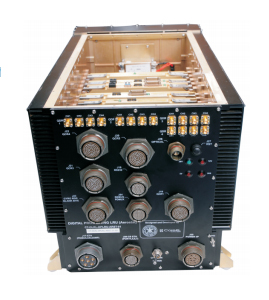
\includegraphics[width=0.3\paperwidth]{LRU.jpg}
            \caption{LRU}
            \label{fig:lru}
        \end{figure}
    \end{column}
    
    \begin{column}{0.45\paperwidth}
        \begin{figure}
            \centering
            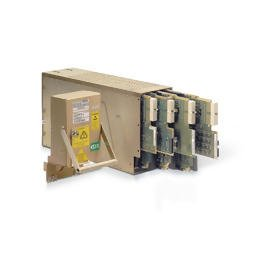
\includegraphics[width=0.3\paperwidth]{IMA.jpg}
            \caption{IMA}
			\label{fig:ima}
        \end{figure}
    \end{column}
  
  \end{columns}
  
\end{frame}

\begin{frame}[t]{Expliquons le titre\ldots} 
  
  \begin{center}
    \begin{mdframed}[style=yellowbox]
      {\small\textcolor{lightgray}{How to address} certification for multi-core based IMA \textcolor{lightgray}{platforms :
       current status and potential solutions}}
       \end{mdframed}
  \end{center}
	
  	\begin{block}{Certification}
  		Méthodologie formelle de tests et documentation des mécanismes de sécurité,
		technique ou non-technique, dans un environnement donné et en utilisant des
		critères établis
  	\end{block}\pause

	\begin{block}{Système certifié en avionique}
	 Système qui répond à des \textbf{standards/normes} de sûreté et de sécurité.
	\end{block}

	% \begin{itemize}
	% 	\item[\faLightbulbO] ISO est une norme 
	% \end{itemize}

\end{frame}

\begin{frame}[t]{Expliquons le titre\ldots}
\begin{center}
    \begin{mdframed}[style=yellowbox]
      {\small\textcolor{lightgray}{How to address} certification for multi-core based IMA \textcolor{lightgray}{platforms :
       current status and potential solutions}}
       \end{mdframed}
  \end{center}

  La certification est délivrée par des agences.

  \begin{figure}
  	\centering
  	
\includegraphics[width=0.8\linewidth]{federal.png}
  	\label{fig:federal}
  \end{figure}
  
\end{frame}

\begin{frame}{Canaux d'interférences}
	Canaux d'interférences \textit{software} et \textit{hardware} entre les partitions
	dans un AMI multi-coeurs
	\bigskip
	\begin{figure}
		\centering
		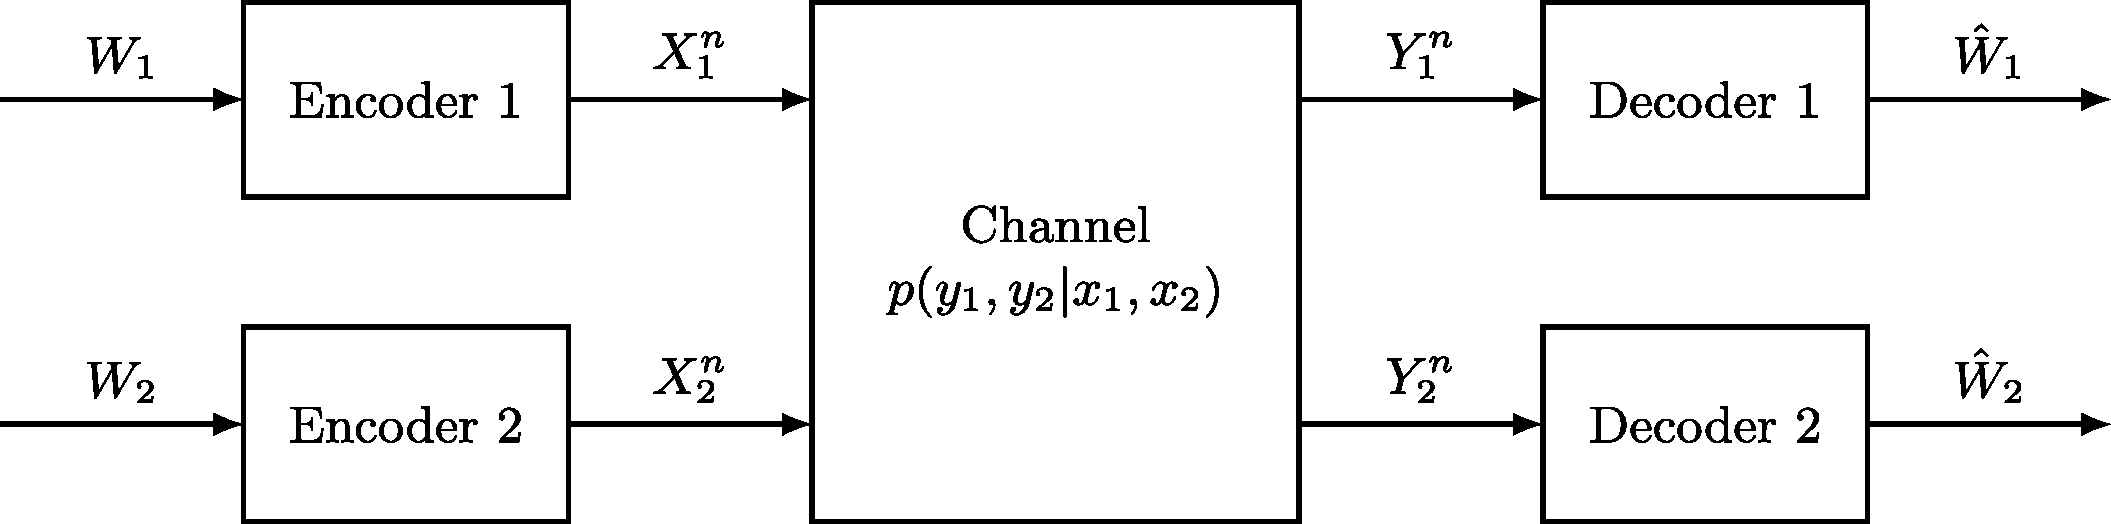
\includegraphics[width=\linewidth]{Interference_channel_model.pdf}
		\caption{Source : Wikipedia \cite{wiki:Interference_channel}}
		\label{fig:Interference_channel_model}
	\end{figure}
\end{frame}


\begin{frame}{Problématique} 

	\begin{block}{Problématique de l'article}
	Peut-on atteindre une meilleure performance et le même niveau de déterminisme qu'un AMI mono-coeur sur un 
	AMI multi-coeurs ?
	\end{block}

	  Enjeux : \pause
  \begin{columns}
	  \begin{column}{0.45\textwidth}
		  \begin{itemize}
		  	\item Performance CPU \pause
			\item Ressources mémoires\pause
			\item Bande passante I/O \pause
			\item Sûreté suffisante \pause
		  \end{itemize}
	  \end{column}
	  \begin{column}{0.45\textwidth}
		  \begin{itemize}
			  \item Comportement déterministe et prédisible \pause
		      \item Partitionnement temps CPU et de ressources sûr \pause
			  \item Certifiable
		  \end{itemize}
	  \end{column}
  \end{columns}
 
\end{frame}

\section[Certification]{Que prendre en compte pour la certification?}%
\label{sec:certification}
 
\begin{frame}{Certification de processeur multi-coeurs}
	Jusqu'à aujourd'hui :\pause
	\begin{itemize}
		\item processeur mono-coeur\pause
		\item architecture RISC\pause
		\item beaucoup de \textit{In Service Experience}\pause
	\end{itemize}
	Avec les nouveaux AMI :\pause
	\begin{itemize}
		\item processeurs multi-coeur\pause
		\item mêmes fonctionnalités que mono-coeur\pause
		\item + communication inter-processeurs / parallélisation / ajout de caches...\pause
		\item peu de documentation car technologies récentes\pause
		\item[$\rightarrow$] difficiles à certifier
	\end{itemize}
\end{frame}

\begin{frame}{Détection d'erreurs et correction}
	\begin{itemize}
		\item Les processeurs multi-coeurs sont plus sensibles aux interférences\pause
		\item Besoin d'une protection ECC (Error Correction Code)\pause
		\item Redondance afin de minimiser les erreurs
	\end{itemize}
\end{frame}

\begin{frame}{Partionnement du temps et des ressources}
	\begin{itemize}
		\item Pas de différence majeure pour le partitionnement des ressources entre mono
			et multi-coeurs\pause
		\item Pour le partitionnement du temps c'est plus compliqué :\pause
			\begin{itemize}
				\item Sur un mono-coeur : un seul thread à la fois, qui peut être
					interrompu\pause
				\item Sur un multi-coeur, éxecution concurrente donc interférences entre
					processus
			\end{itemize}
	\end{itemize}
\end{frame}

\section[CI physiques]{Canaux d'interférences physiques}

\begin{frame}{Architecture d'un processeur AMI multi-coeur}
	\begin{figure}
		\centering
		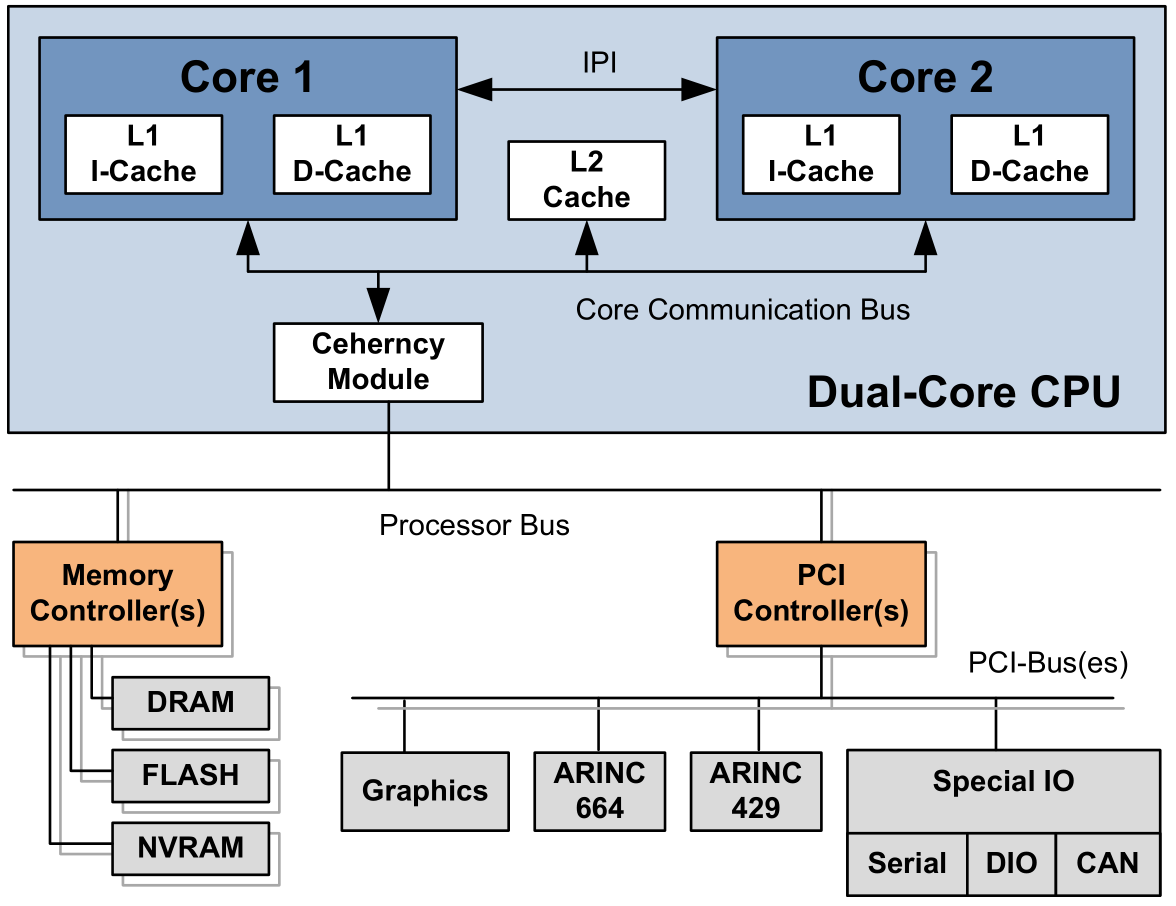
\includegraphics[width=0.7\linewidth]{arch.png}
		\caption{Architecture d'un CPU deux coeurs \cite{Fuch}}
		\label{fig:arch}
	\end{figure}	
\end{frame}

\begin{frame}{Caches}

			\begin{figure}
				\centering
				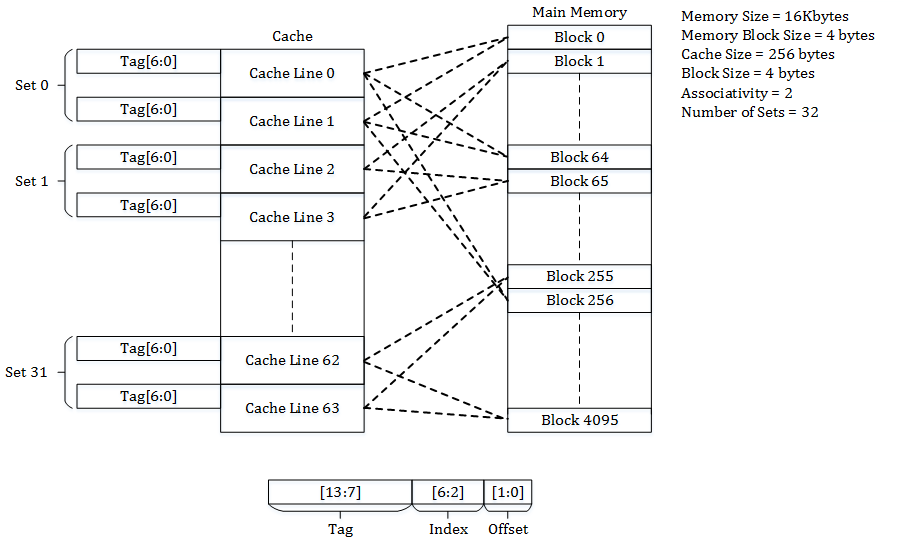
\includegraphics[width=\linewidth]{Set-Associative_Cache_Snehal_Img.png}
				\caption{Exemple de cache set-associatif \cite{wiki:Cache_placement_policies}}
				\label{fig:Set-Asso}
			\end{figure}
\end{frame}

\begin{frame}{Partage de cache}
	Comparaison :\pause
	\begin{itemize}
		\item Processeur Intel :
			\begin{itemize}
				\item Cache L1 64Kbyte par processeur
				\item Cache L2 2Mbyte \textbf{partagée}
			\end{itemize}\pause
		\item Processeur AMD :
			\begin{itemize}
				\item Cache L1 128Kbyte par processeur
				\item Cache L2 512Kbyte \textbf{par processeur}
			\end{itemize}\pause
	\end{itemize}
	\begin{itemize}
		\item[$\rightarrow$] Input : données de taille variables que les processeurs
			lisent ou modifient
		\item[$\rightarrow$] On mesure le thoughput\pause
	\end{itemize}
	\medskip
\end{frame}

\begin{frame}{Partage de cache}

	% \hspace{0.2cm}{\tiny L1 = 64Kbytes/L1 + L2 $\simeq$ 2Mbytes \hspace{2.1cm} L1 = 128Kbytes/L1+ L2 $\simeq$
	% 750Kbytes} \\
	% \hspace{0.2cm}{\tiny L2 partagée \hspace{4.67cm} L2 non-partagée}
	\begin{center}
		\begingroup
		\footnotesize
		\begin{tabular}{r|ccc}
		& L1 & L1 + L2 & Cache L2 partagée \\
		\hline
			Intel & 64Kbytes & 2Mbytes & Oui \\
			AMD & 128Kbytes & 750Kbytes & Non \\
		\end{tabular}
		\endgroup
	\end{center}

	\begin{figure}
		\centering
		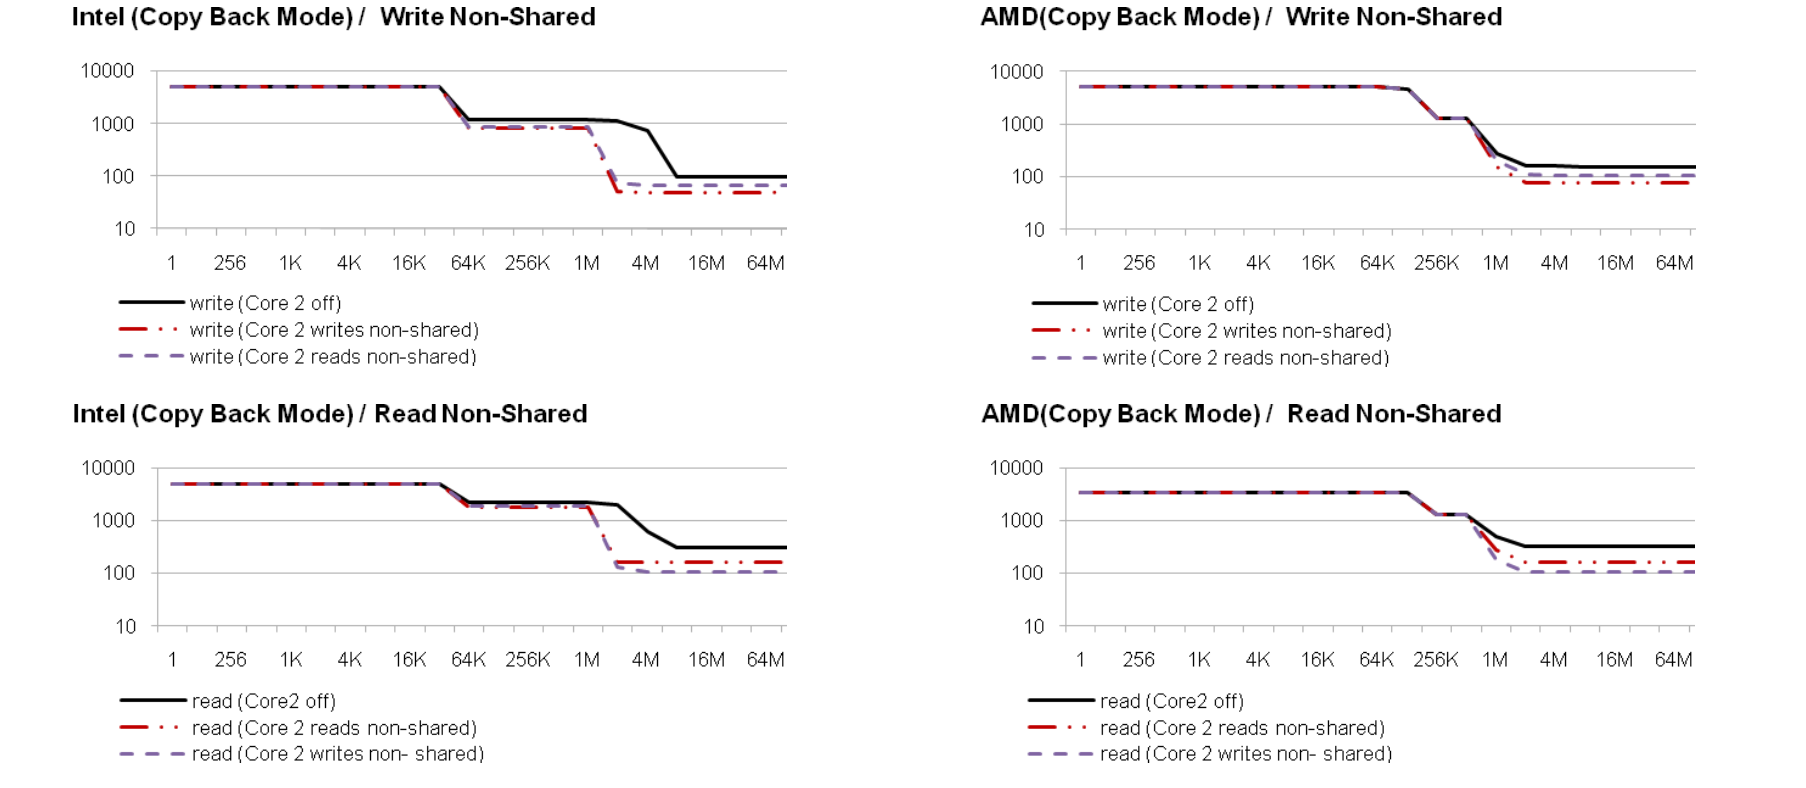
\includegraphics[width=0.9\paperwidth]{results_cache_sharing.png}
		\caption{Résultats \cite{Fuch}}
		\label{fig:results_cache_sharing}
	\end{figure}	
\end{frame}

\begin{frame}{Cohérence de cache}
	\begin{itemize}
		\item Protocole MSI (Modified, Shared, Invalid)
	\end{itemize}
	\begin{figure}
		\centering
		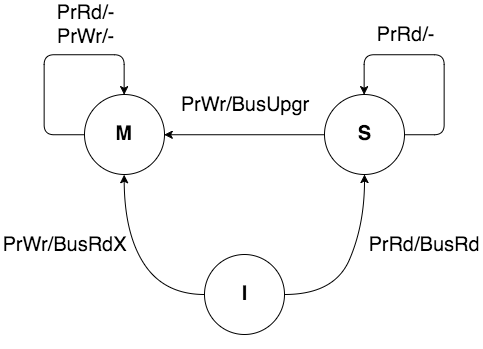
\includegraphics[width=0.6\linewidth]{State_diagram_for_processor_transactions.png}
		\caption{Transitions entre états d'une ligne de cache \cite{wiki:MSI_protocol}}
		\label{fig:State_di}
	\end{figure}
\end{frame}

\begin{frame}{Cohérence de cache}

	% \hspace{0.2cm}{\small\textbf{Intel :} L1 = 64Kbytes/ L1 + L2 $\simeq$ 2Mbytes / L2 partagée } \\
	
	% \hspace{0.2cm}{\small\textbf{AMD :} L1 = 128Kbytes/ L1+ L2 $\simeq$ 750Kbytes / L2 non-partagée}

	\begin{center}
		\begin{tabular}{r|ccc}
		& L1 & L1 + L2 & Cache L2 partagée \\
		\hline
			Intel & 64Kbytes & 2Mbytes & Oui \\
			AMD & 128Kbytes & 750Kbytes & Non \\
		\end{tabular}
	\end{center}

	\begin{figure}
		\centering
		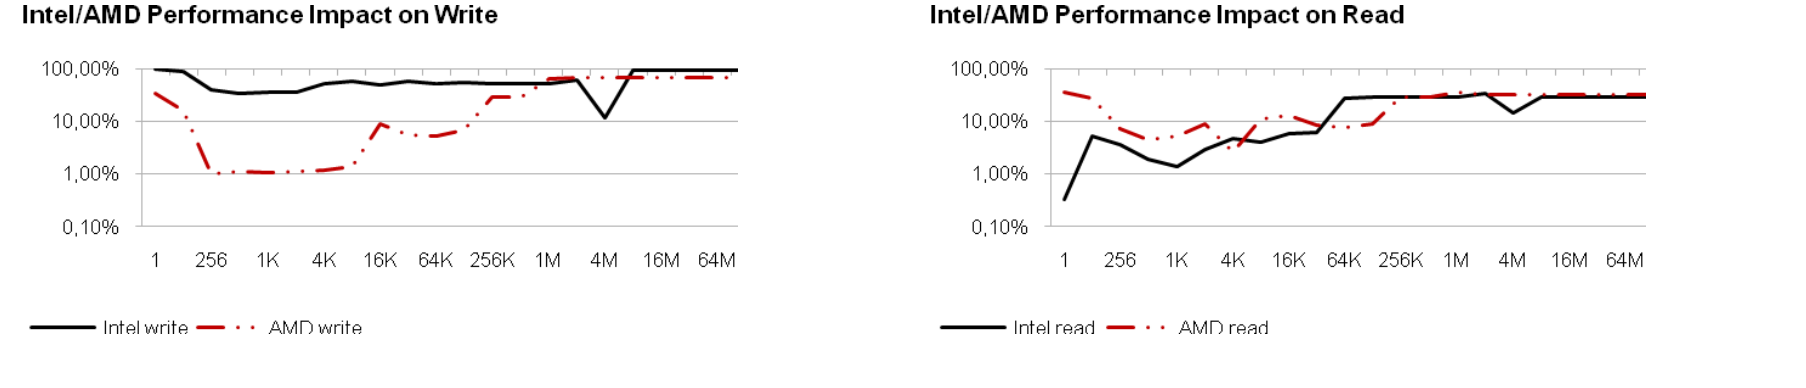
\includegraphics[width=0.9\paperwidth]{results_performance_coherency.png}
		\caption{Résultats \cite{Fuch}}
		\label{fig:results_cache_sharing}
	\end{figure}	
\end{frame}

\begin{frame}{Bus, I/O Devices, et Interruptions}
	\begin{itemize}
		\item Bande passante de bus partagée, performance réduite si les données sont trop
			grandes (> taille de cache)\pause
		\item I/O Devices : une requête à la fois donc bien choisir les bus de
			communication (PCI, etc)\pause
		\item Interruptions : un processeur doit avertir l'autre s'il existe un seul même
			ligne d'interruption
	\end{itemize}
\end{frame}

\section[CI logiciels]{Canaux d'interférence logiciels}

\begin{frame}{Concepts}
	\begin{itemize}
		\item la configuration software (partitions, etc.) doit s'adapter au processeur
		\item les modules AMI doivent distribuer un bande passante \textbf{élevée} et
			\textbf{constante} aux différentes applications en fonction du partitionnement
			de temps
	\end{itemize}
\end{frame}

\begin{frame}{Concepts}
	\begin{columns}
		\begingroup
		\small
		\hspace{0.3cm}
		\begin{column}{0.55\paperwidth}
			Approche AMP (asymmetric multi\-processing) :
				\begin{itemize}
					\item[$+$] le software n'a pas besoin de savoir que le processeur est
						multi-coeur
					\item[$+$] software optimisé pour la tâche associée
					\item[$-$] instances certifiée au niveau maximum car elles ont un
						processeur exclusif 
					\item[$-$] partitionnement ressources simplifié
					\item[$-$] synchronisation entre tâche plus complexe
				\end{itemize}
		\end{column}
		\endgroup
		\begin{column}{0.45\paperwidth}
			\begin{figure}
				\centering
				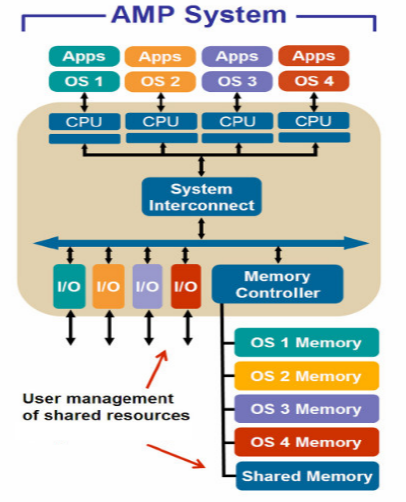
\includegraphics[width=0.7\linewidth]{amp.png}
			\end{figure}	
		\end{column}
	\end{columns}
\end{frame}

\begin{frame}{Concepts}
	\begin{columns}
		\begingroup
		\small
		\hspace{0.3cm}
		\begin{column}{0.55\paperwidth}
			Approche SMP (symmetric multi\-processing) :
				\begin{itemize}
					\item[$+$] un seul OS / une seule configuration
					\item[$+$] isolation totale des tâches critiques
					\item[$-$] meilleure balance de charge (load-balancing)
					\item[$-$] software plus complexe
					\item[$-$] faux partages en cache
					\item[$-$] plus d'interférences
				\end{itemize}
		\end{column}
		\endgroup
		\begin{column}{0.45\paperwidth}
			\begin{figure}
				\centering
				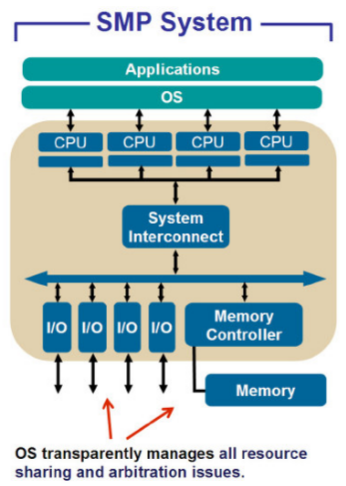
\includegraphics[width=0.7\linewidth]{smp.png}
			\end{figure}	
		\end{column}
	\end{columns}
\end{frame}

\begin{frame}{Concepts}
	\begin{itemize}
		\item Parallélisation par threads :
			\begin{itemize}
				\item[$+$] plus de contrôle sur les tâches
				\item[$-$] données partagées donc faux partage possible 
			\end{itemize}
		\item Parallélisation par instruction :
			\begin{itemize}
				\item[$+$] OpenMP permet de répartir un calcul sur plusieurs coeurs
				\item[$-$] données partagées donc faux partage possible 
			\end{itemize}
	\end{itemize}
\end{frame}

\begin{frame}{Approche SMP pour les AMI}
	\begin{itemize}
		\item De plus en plus d'application qui demandent une haute performance avec un
			bas niveau de criticité
		\item Mais comment faire rouler une application de haute criticité (sûreté) à côté
			d'une application de basse criticité sans avoir d'interférences ?
		\item Une solution : PikeOS
	\end{itemize}	
\end{frame}

\begin{frame}{Approche SMP pour les AMI}
	\begin{figure}
		\centering
		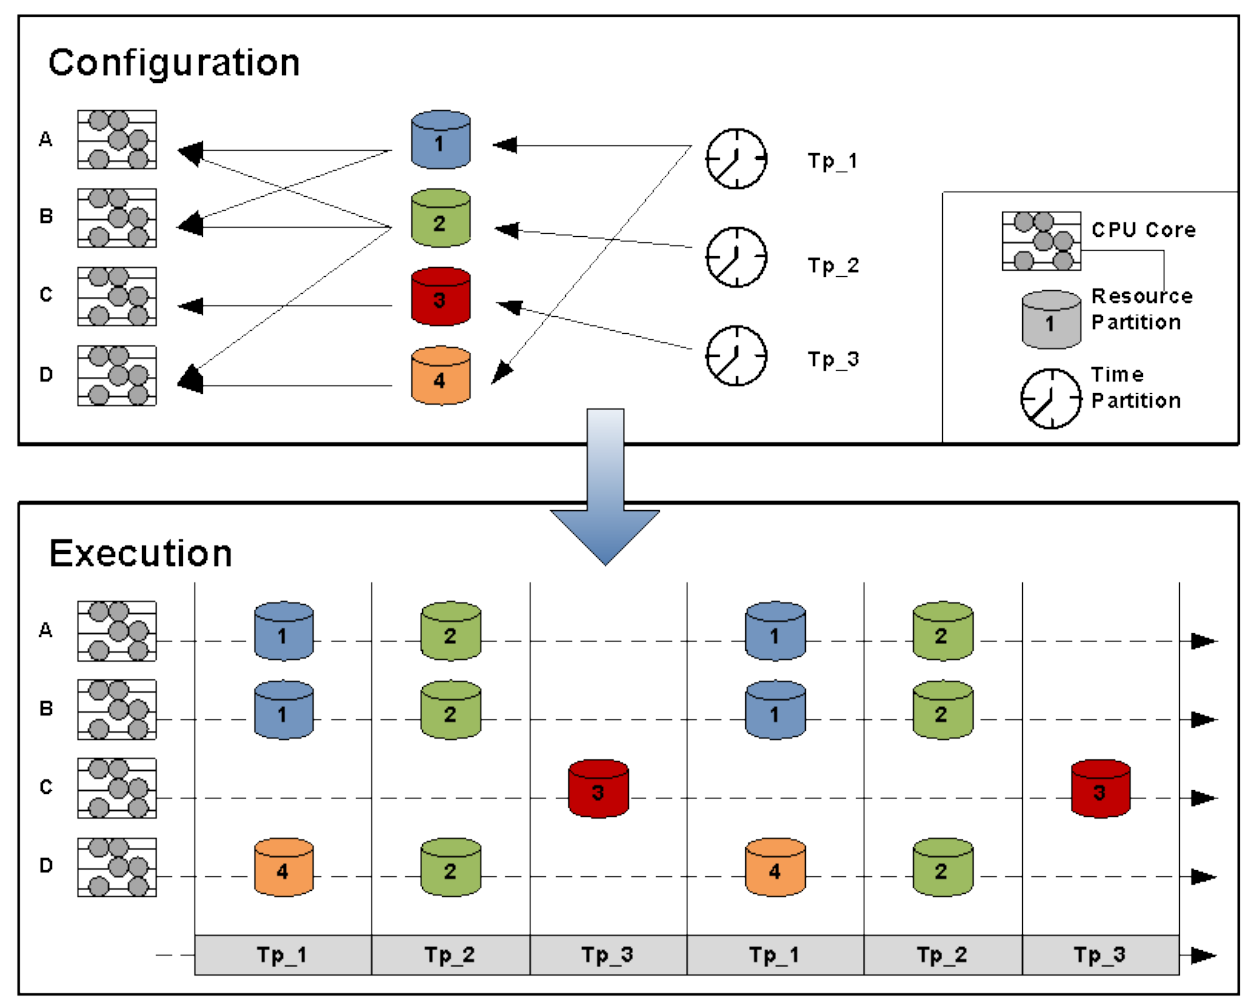
\includegraphics[height=0.6\paperheight]{pikeos.png}
		\caption{Exemple de configuration et d'exécution avec PikeOS \cite{Fuch}}
		\label{fig:pikeos}
	\end{figure}
\end{frame}

\section{Conclusion}

\begin{frame}{Conclusion}
	\begin{itemize}
		\item Les CPUs multi-coeurs vont devenir une nécéssité dans l'avionique\pause
		\item Besoin de \textit{In Service Experience} sur des systèmes \textbf{moins
			critiques}\pause
		\item Besoin d'un design réfléchi et examiné au plus près \pause
		\item Choix de processeur\pause
		\item[$\rightarrow$] Systèmes plus sûrs\pause
	\end{itemize}

	\begin{center}
		\textcolor{polymtlred}{Merci !}
	\end{center}
\end{frame}

\setbeamertemplate{bibliography item}{\insertbiblabel}
\begin{frame}[allowframebreaks]
        \frametitle{References}
        \bibliographystyle{plain}
        \bibliography{./biblio.bib}
\end{frame}

\end{document}

% vim: set ts=4 sw=4 tw=90 noet :
